\chapter{SOLID}

\section{Analyse Single-Responsibility-Principle (SRP)}
\subsection{Positiv-Beispiel}
Die nachfolgende Abbildung zeigt das gekürzte UML-Diagramm der Klasse
\textit{CollectAction}. Die ist in der Schicht \textit{plugins}
angesiedelt. Sie implementiert das \textit{IAction}-Interface, welche
vom Spieler initiierte Aktionen darstellt. Die einzige Aufgabe der
\textit{CollectAction} ist es, zu prüfen, ob ein Item unter dem 
Spieler liegt und dieses aufzunehmen bzw. mit dem bisherigen Item
gleichen Typ (z.B. Rüstung) auszutauschen. Dafür bekommt es ein
\textit{Game}-Objekt übergeben, aus welchem die nötigen Informationen
gezogen und die nötigen Funktionen aufgerufen werden können.

\vspace{0.5cm}
\begin{figure}[H]
    \centering
    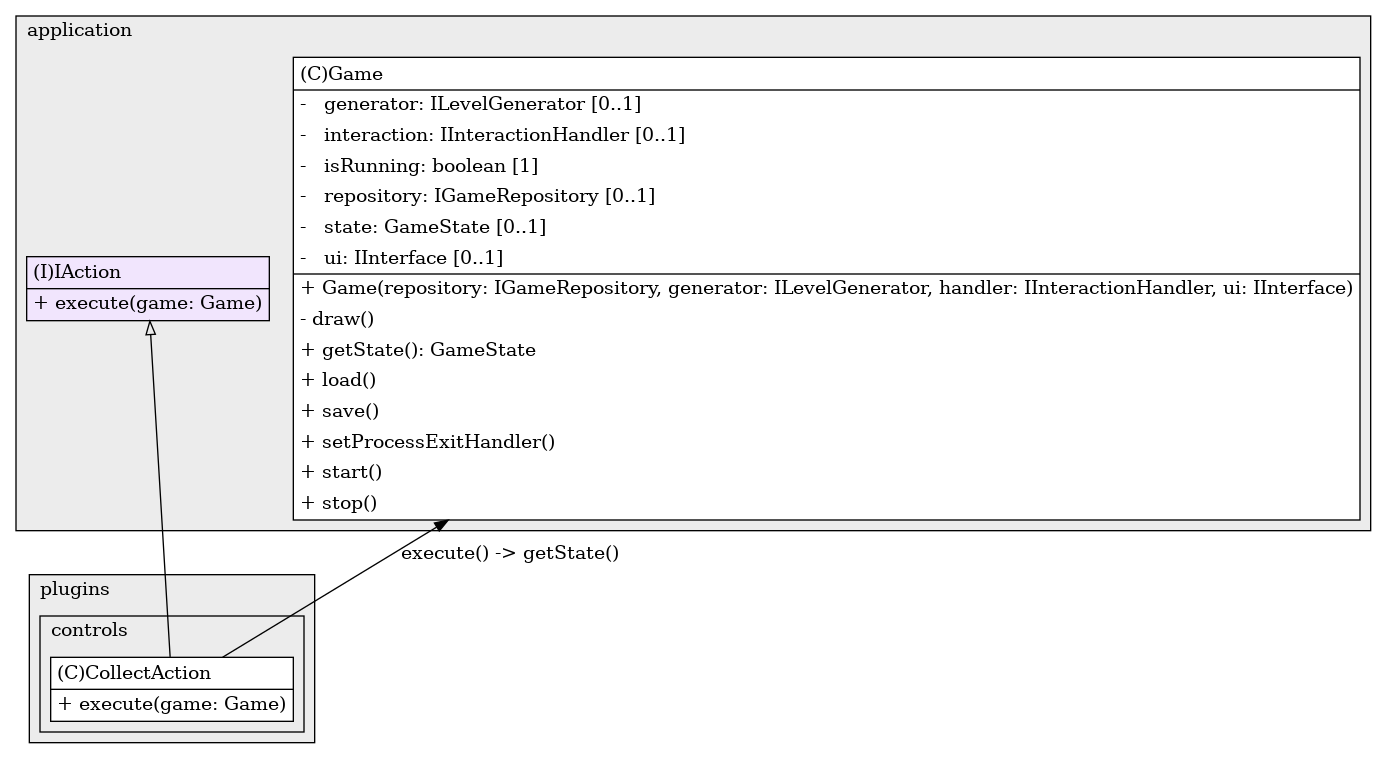
\includegraphics[width=1\linewidth]{Bilder/Visualisierung/CollectActionSimplified_structure.png}
    \caption{Analyse Single-Responsibility-Principle: Positiv}
\end{figure}

\subsection{Negativ-Beispiel}

\section{Analyse Open-Closed-Principle (OCP)}

\section{Analyse Dependency-Inversion-Principle (DIP)}